\documentclass[a4paper]{article}
\usepackage[utf8]{inputenc}
\usepackage[russian,english]{babel}
\usepackage[T2A]{fontenc}
\usepackage[left=10mm, top=20mm, right=18mm, bottom=15mm, footskip=10mm]{geometry}
\usepackage{indentfirst}
\usepackage{amsmath,amssymb}
\usepackage[italicdiff]{physics}
\usepackage{graphicx}
\graphicspath{{images/}}
\DeclareGraphicsExtensions{.pdf,.png,.jpg}
\usepackage{wrapfig}
\usepackage{pgfplots}

\usepackage{caption}
\captionsetup[figure]{name=Рисунок}
\captionsetup[table]{name=Таблица}


\title{\underline{Лабораторная работы 1.4.8}}
\author{Старостин Александр, Б01-401}
\date {29 Октября, 2024 год}


\begin{document}

\maketitle
\newpage

\textbf{Измерение модуля Юнга методом аккустического резонанса}

\section{Аннотация}
    \par \textbf{Цель работы:} исследовать явление акустического резонанса в тонком стержне; измерить скорость распространения продольных звуковых колебаний в тонких стержнях из различных материалов и различных размеров; измерить модули Юнга различных материалов.\\

    \par \textbf{В работе используются:} генератор звуковых частот, частотомер, осциллограф, электромагнитные излучатель и приёмник колебаний, набор стержней из различных материалов.

\section{Теоретические сведения}

Скорость $u$ распространения продольной акустической волны в середе зависит от плотности среды $p$ и модуля Юнга $E$, как:

\begin{equation}
	u = \sqrt{\frac{E}{p}}
\end{equation}

Зная номер гармоники $n$ и соответствующую ей резонансную частоту $f_n$, на которой наблюдается усиление амплитуды колебаний, можно вычислить скорость распространения продольных волн в стержне длиной $L$:

\begin{equation}
	u = \frac{2 L f_n}{n}
\end{equation}

\section{Ход работы}

\subsection{Настройка осциллографа и звукового генератора}
\item В ходе работы был ознакомлен с основными органами управления электронного осциллографа. Провёл предварительную настройку осциллографа и звукового генератора.

\subsection{Установка металлических стержней}
\item Раздвинул датчики и поместил по очереди между ними исследуемые стержени: медный, стальной и дюралюминевый. Длина стержней составляет: $L = 60.0\pm0.1 $см.

\subsection{Правильное размещение электромагнитов}
\item Разместил электромагниты напротив торцов стержня так, чтобы
торцы стержня совпали с центрами датчиков, а зазор между полюсами электромагнита и торцевой поверхностью стержней составлял 1–3 мм. Плоскость магнитов направил строго перпендикулярно оси стержня, не допустив соприкосновения электромагнита с торцами стержня.

\subsection{Определение диапозонов частот первого резонанса}
\item По формуле (2) посчитал первые резонансные частоты для стрежней, используя табличные значения скоростей звука в метталах:


\begin{table}[h!]
\centering
\caption{Частоты первого резонанса}
\begin{tabular}{|c|c|c|c|}
\hline
Величина & Медь & Сталь & Дюралюминий \\ \hline
Скорости звука $u$, м/c & $3710$ & $5170$ & $5080$ \\ \hline
Частоты $f_1$, Гц & $3092$ & $4308$ & $4233$ \\ \hline
\end{tabular}
\end{table}

\subsection{Поиск первого резонанса}

\item Медленно перестроив звуковой генератор вблизи расчетной частоты $f_1$ нашёл первый резонанс, наблюдав за амплитудой колебаний на
экране осциллографа. При приближении к резонансу амплитуда сигнала с
регистрирующего датчика (канал CH2) резко возрастала, а амплитуда опорного сигнала (канал CH1) не изменялась.

\subsection{Измерение первого резонанса и вычисление погрешности измерения}

\item Определил значение первой резонансной частоты $f_1$ по индикатору
частотомера..

\begin{table}[h!]
\centering
\caption{Измерения первой резонансной частоты}
\begin{tabular}{|c|c|c|c|c|c|}
\hline
N & 1 &2 &3 &4 &5\\ \hline
Медь, Гц & 3249 & 3247 & 3255 & 3233 & 3255 \\ \hline
\end{tabular}
\end{table}

\item Погрешность измерения резонансной частоты: $\sigma_f = \sqrt{\frac{1}{N(N-1)}\sum_{1}^{N}(f_i-\overline{f})^2} = 4 Гц$


\subsection{Измерение резонансных частот}
\item Получил резонансы на частотах, соответствующих следующим
(кратным) гармоникам. Для этого, плавно перестроив генератор, добился резонанса вблизи частот $f_n = nf_1$, где n = 2, 3, ..., 7.

\begin{table}[h!]
\centering
\caption{Частоты резонанса}
\begin{tabular}{|c|c|c|c|}
\hline
N & Медь, Гц & Сталь, Гц & Дюралюминий, Гц \\ \hline
1 & 3249 & 4126 & 4255 \\ \hline
2 & 6475 & 8241 & 8500 \\ \hline
3 & 9762 & 12394 & 12761 \\ \hline
4 & 12956 & 16524 & 17022 \\ \hline
5 & 16213 & 20649 & 21275 \\ \hline
6 & 19470 & 24770 & 25533 \\ \hline
7 & 22772 & 28892 & 29785 \\ \hline
\end{tabular}
\end{table}






\subsection{Определение плотностей материалов}

\begin{table}[h!]
\centering
\caption{Медь}
\begin{tabular}{|c|c|c|c|c|c|}
\hline
N/Медь & Длина, см & Диаметр, см & Площадь, см^2 & Масса, г & Плотность, кг/м^3 \\ \hline
1 & $3.03\pm0.01$ & $1.246\pm0.001$ & $1.219\pm0.002$ & $30.115\pm0.003$ &8155.2\\ \hline
2 & $2.97\pm0.01$ & $1.185\pm0.001$ & $1.102\pm0.002$ & $29.119\pm0.003$ &8894.3 \\ \hline
3 & $3.01\pm0.01$ & $1.184\pm0.001$ & $1.100\pm0.002$ & $29.459\pm0.003$ &8893.6\\ \hline
4 & $4.14\pm0.01$ & $1.240\pm0.001$ & $1.207\pm0.002$ & $41.349\pm0.003$ &8274.7\\ \hline
5 & $4.05\pm0.01$ & $1.242\pm0.001$ & $1.211\pm0.002$ & $40.361\pm0.003$ &8229.9\\ \hline
6 & $4.00\pm0.01$ & $1.212\pm0.001$ & $1.153\pm0.002$ & $41.007\pm0.003$ &8890.4\\ \hline
7 & $3.95\pm0.01$ & $1.242\pm0.001$ & $1.211\pm0.002$ & $39.391\pm0.003$ &8235,4\\ \hline
8 & $4.03\pm0.01$ & $1.171\pm0.001$ & $1.076\pm0.002$ & $38.723\pm0.003$ &8926,5\\ \hline
\end{tabular}
\end{table}

\item $\overline{p} = 8562.4$ кг/м$^3$.
\item $\varepsilon_{p} = \varepsilon_{p}^\text{приб} = \sqrt{\left( \dfrac{\sigma_{m}}{m}\right)^2 + \left(\dfrac{\sigma_l}{l_\text{min}}\right)^2+4\left(\dfrac{\sigma_D}{D_\text{min}}\right)^2} \approx 3.9\% $

\begin{table}[h!]
\centering
\caption{Сталь}
\begin{tabular}{|c|c|c|c|c|c|}
\hline

N/Медь & Длина, см & Диаметр, см & Площадь, см^2 & Масса, г & Плотность, кг/м^3 \\ \hline
1 & $3.98\pm0.01$ & $1.198\pm0.001$ & $1.126\pm0.002$ & $35.200\pm0.003$ &7850.1\\ \hline
2 & $2.96\pm0.01$ & $1.199\pm0.001$ & $1.129\pm0.002$ & $26.036\pm0.003$ &7794.3\\ \hline
3 & $2.97\pm0.01$ & $1.197\pm0.001$ & $1.125\pm0.002$ & $26.163\pm0.003$ &7832.0\\ \hline
4 & $3.13\pm0.01$ & $1.180\pm0.001$ & $1.093\pm0.002$ & $28.118\pm0.003$ &8218.8\\ \hline
5 & $4.10\pm0.01$ & $1.224\pm0.001$ & $1.176\pm0.002$ & $36.927\pm0.003$ &7658.2\\ \hline
6 & $4.00\pm0.01$ & $1.199\pm0.001$ & $1.129\pm0.002$ & $35.153\pm0.003$ &7787.4\\ \hline
7 & $4.13\pm0.01$ & $1.203\pm0.001$ & $1.136\pm0.002$ & $37.102\pm0.003$ &7907.6\\ \hline
8 & $3.97\pm0.01$ & $1.200\pm0.001$ & $1.130\pm0.002$ & $34.950\pm0.003$ &7788.0\\ \hline
\end{tabular}
\end{table}

\item $\overline{p} = 7854.6$ кг/м$^3$.
\item $\varepsilon_{p} = \varepsilon_{p}^\text{приб} = \sqrt{\left( \dfrac{\sigma_{m}}{m}\right)^2 + \left(\dfrac{\sigma_l}{l_\text{min}}\right)^2+4\left(\dfrac{\sigma_D}{D_\text{min}}\right)^2} \approx 3.9\% $







\begin{table}[h!]
\centering
\caption{Дюралюминий}
\begin{tabular}{|c|c|c|c|c|c|}
\hline
N/Медь & Длина, см & Диаметр, см & Площадь, см^2 & Масса, г & Плотность, кг/м^3 \\ \hline
1 & $3.08\pm0.01$ & $1.174\pm0.001$ & $1.082\pm0.002$ & $9.267\pm0.003$ &2779.5\\ \hline
2 & $3.02\pm0.01$ & $1.175\pm0.001$ & $1.084\pm0.002$ & $8.995\pm0.003$ &2746.8 \\ \hline
3 & $3.01\pm0.01$ & $1.205\pm0.001$ & $1.140\pm0.002$ & $9.491\pm0.003$ &2764.9\\ \hline
4 & $3.02\pm0.01$ & $1.186\pm0.001$ & $1.104\pm0.002$ & $9.199\pm0.003$ &2757.2\\ \hline
5 & $4.13\pm0.01$ & $1.174\pm0.001$ & $1.082\pm0.002$ & $12.459\pm0.003$ &2786.8\\ \hline
6 & $4.00\pm0.01$ & $1.182\pm0.001$ & $1.097\pm0.002$ & $12.185\pm0.003$ &2776.1\\ \hline
7 & $4.12\pm0.01$ & $1.218\pm0.001$ & $1.165\pm0.002$ & $13.236\pm0.003$ &2757.2\\ \hline
8 & $4.15\pm0.01$ & $1.127\pm0.001$ & $0.997\pm0.002$ & $12.485\pm0.003$ &3015.8\\ \hline
\end{tabular}
\end{table}

\item $\overline{p} = 2798.0$ кг/м$^3$.
\item $\varepsilon_{p} = \varepsilon_{p}^\text{приб} = \sqrt{\left( \dfrac{\sigma_{m}}{m}\right)^2 + \left(\dfrac{\sigma_l}{l_\text{min}}\right)^2+4\left(\dfrac{\sigma_D}{D_\text{min}}\right)^2} \approx 3.9\% $





\subsection{Проверка условия тонкого стержня}
\item Медь:
\item $\overline{d} = 1.215 \ $ см
\item $\varepsilon_d = \varepsilon_{d}^\text{приб} = \dfrac{\sigma_d}{\overline{d}} = 0.8\%$
\item

\item Сталь:
\item $\overline{d} = 1.200 \ $ см
\item $\varepsilon_d = \varepsilon_{d}^\text{приб} = \dfrac{\sigma_d}{\overline{d}} = 0.8\%$
\item

\item Дюралюминий:
\item $\overline{d} = 1.180 \ $ см
\item $\varepsilon_d = \varepsilon_{d}^\text{приб} = \dfrac{\sigma_d}{\overline{d}} = 0.8\%$
\item

\item Для всех $\overline{d}$ выполянется, что $\frac{\overline{d}}{2\lambda} << 1$, где $\lambda$ - длина звуковой волны в каждом стержне. Значит, приближение тонкого стержня выполняется.


\subsection{Выполнение измерений и вычислений для стального и диралюминевого стержней}

\item Смотреть все измерения и вычисления для стального и диралюминевого стержней в предыдущих пунктах.



\subsection{Возникновение резонансных колебаний при половинной частоте первого резонанса}

\item Для стержня из дюраля проведёл дополнительный опыт: перестроив генератор, добился возбуждения первой гармоники $f_1$ резонансных
колебаний в стержне при «половинной» частоте генератора $f = \frac{f_1}{2}$, пронаблюдал на экране осциллографа фигуру Лиссажу (в режиме работы
«X–Y») и запечатлил её.

\begin{figure}[!ht]
    \centering
    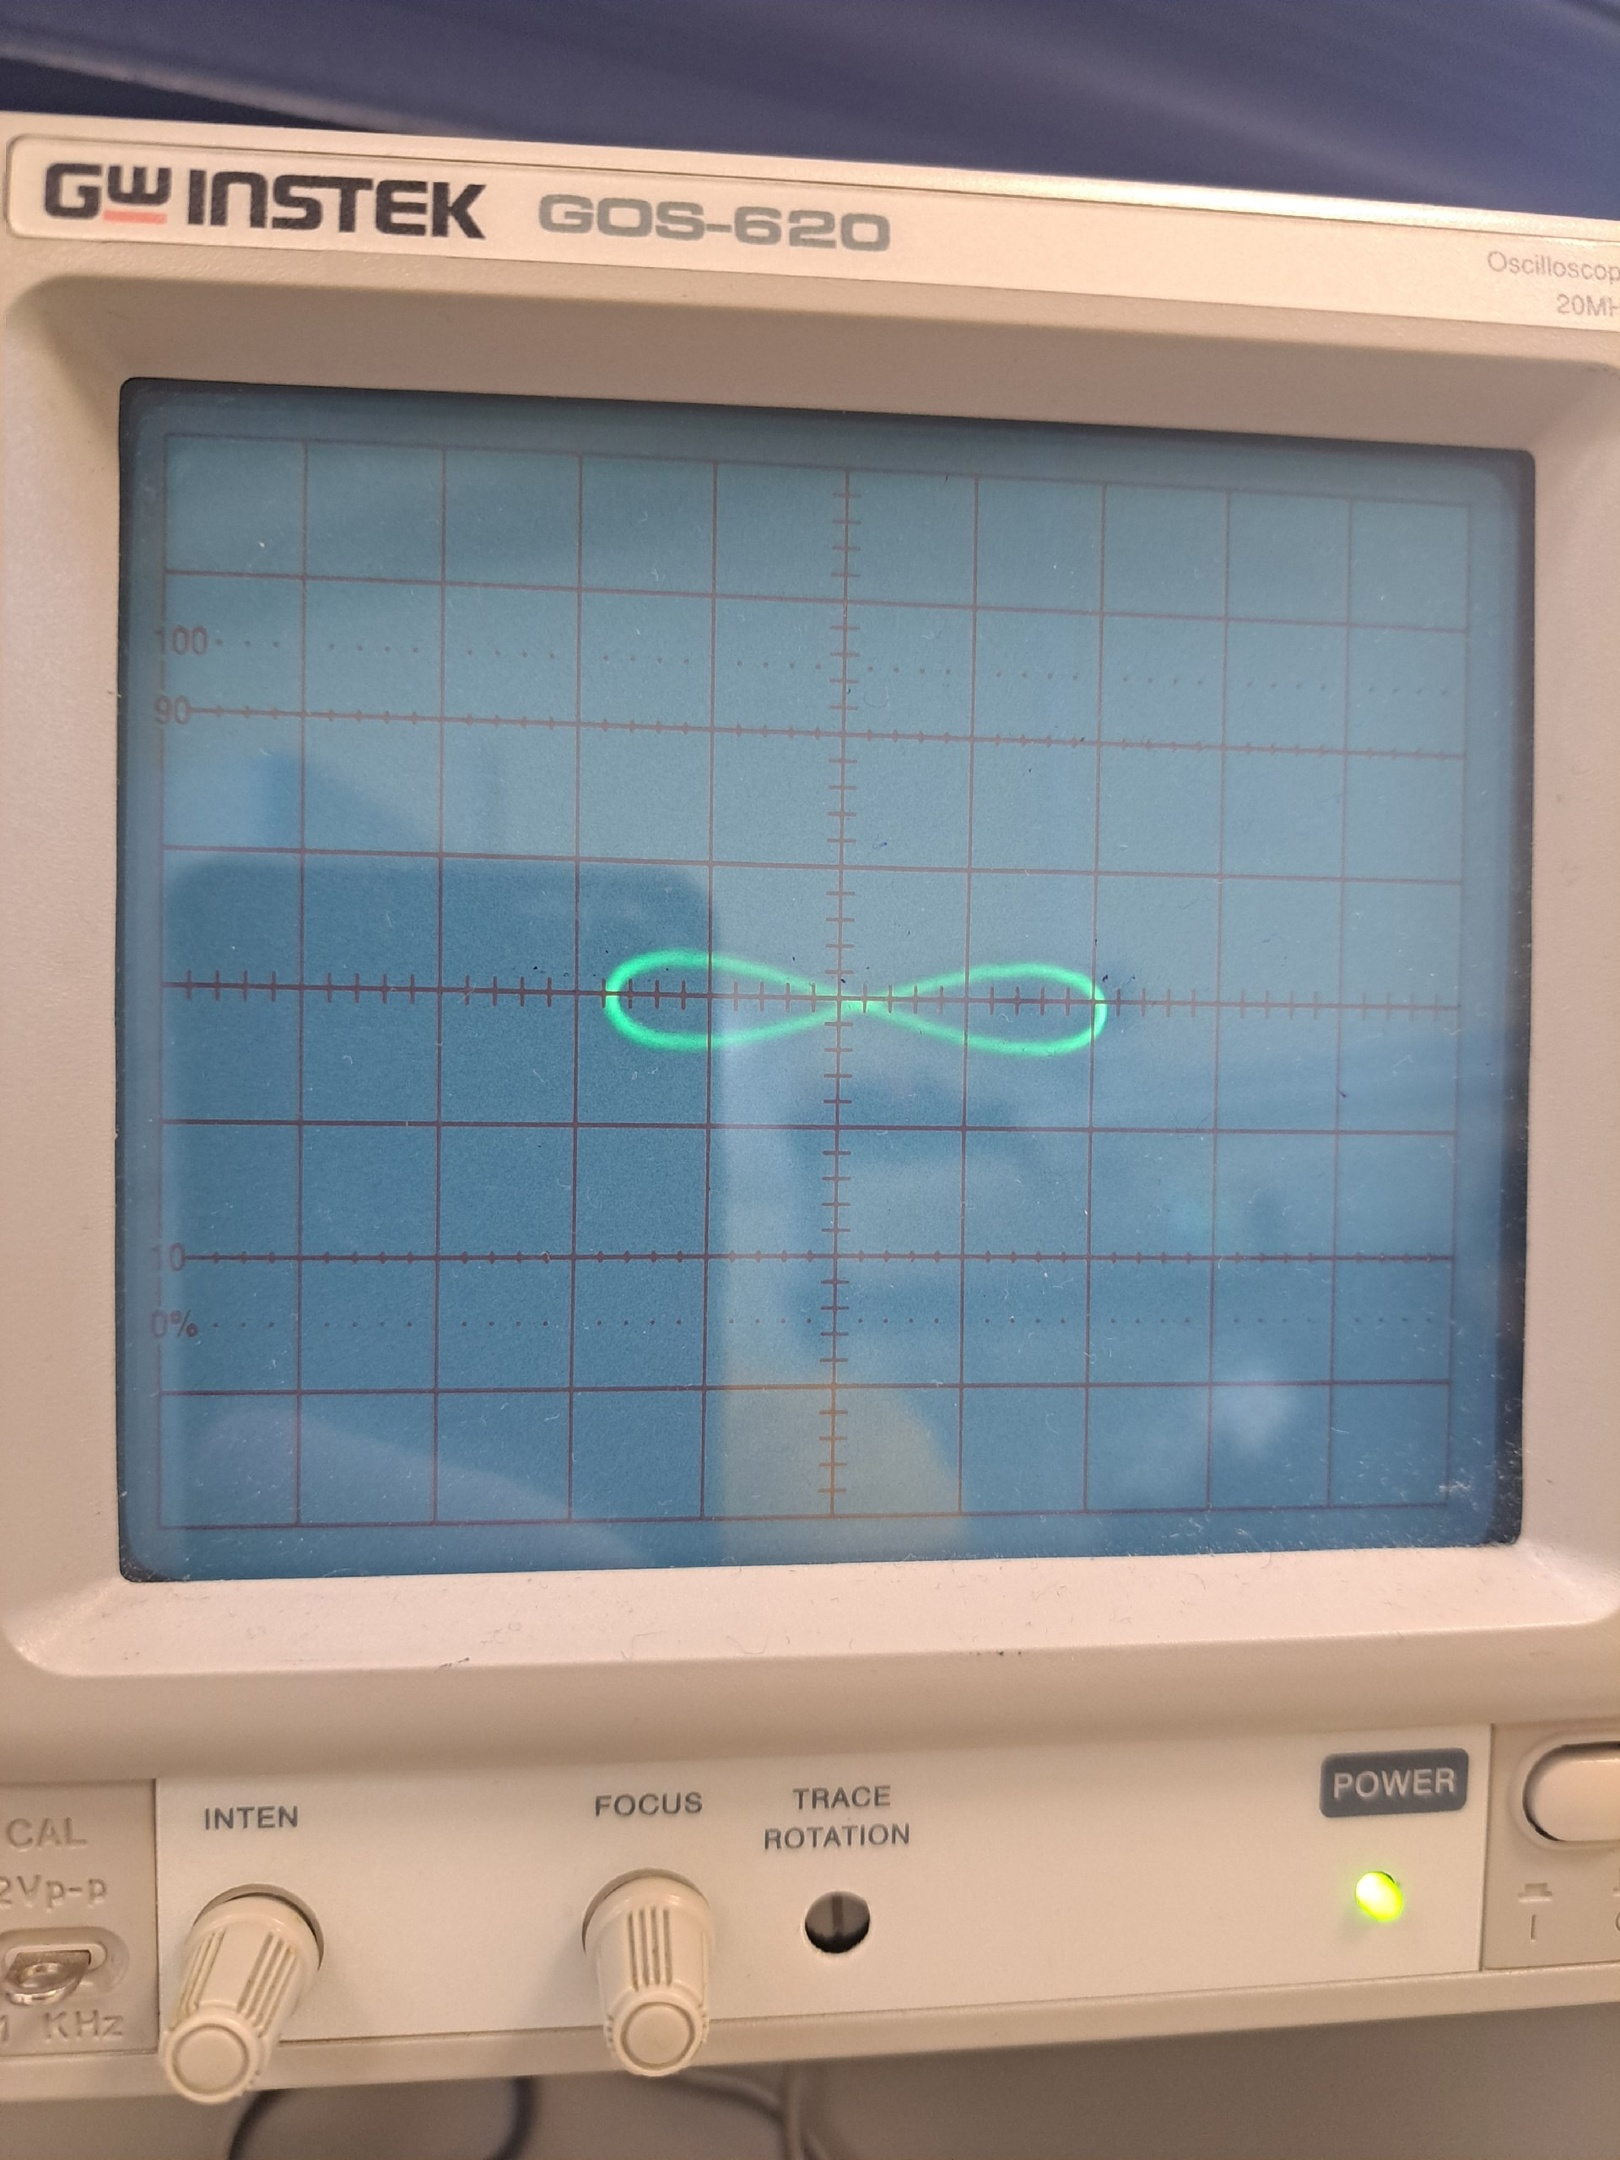
\includegraphics[scale=0.15]{Бабочка.jpg}
    \caption{Фигура Лисасажу ввиде бабочки}
\end{figure}
\item
\item По моему мнению, возникновение резонансных колебаний при данной частоте связано тем, что при половинной частоте внутри стержня помещается ровно половина одной звуковой волны. Тк половина волны повторяет саму волну (вторая половина волны является зеркальным отражением первой), то половина волны заменяет основную волну и является резонансной.

\newpage

\subsection{Определение добротности стержня как колебательной системы}

\begin{table}[h!]
\centering
\caption{}
\begin{tabular}{|c|c|c|c|c|c|}
\hline
№ $N$ \uparrow & $2A$ , дел & $f$, кГц & № $N$ \downarrow & $2A$, дел & $f$, кГц \\ \hline
1 & 8.0 & 3.2551 &1 & 8.0 & 3.2550\\ \hline
2 & 7.8 & 3.25518 &2 & 7.8 & 3.2548\\ \hline
3 & 7.6 & 3.2552 &3 & 7.4 & 3.2547 \\ \hline
4 & 6.8 & 3.2553 &4 & 6.6 & 3.2546 \\ \hline
5 & 6.2 & 3.2554 &5 & 6.0 & 3.2545 \\ \hline
6 & 5.6 & 3.2555 &6 & 5.6 & 3.2544\\ \hline
7 & 5.0 & 3.2556 &7 & 4.8 & 3.2543\\ \hline
8 & 4.6 & 3.2557 &8 & 4.4 & 3.2541\\ \hline
9 & 4.2 & 3.2558 &9 & 3.8 & 3.2540\\ \hline
10 & 3.8 & 3.2559 &10 & 3.4 & 3.2539\\ \hline
11 & 3.4 & 3.256 &11 & 3.2 & 3.2538\\ \hline
12 & 3.2 & 3.2561 &12 & 3.0 & 3.2538\\ \hline
13 & 3.0 & 3.2562 &13 & 2.8 & 3.2536\\ \hline
14 & 2.8 & 3.2563 &14 & 2.6 & 3.2535\\ \hline
15 & 2.6 & 3.2564 &15 & 2.4 & 3.2534\\ \hline
16 & 2.4 & 3.2565 &16 & 2.2 & 3.2534\\ \hline
\end{tabular}
\end{table}

\item Определим добротность стержня как колебательной системы, измерив амплитудно-частотную характеристику одного из стержней $A(f - f_1)$ вблизи первого резонанса.
$Q = \frac{f_A}{f_1 - f_2}$, где $f_1$ и $f_2$ - частоты, соответствующие амплитуде равной $\frac{A}{\sqrt{2}}$
Из таблицы выбираем нужно нам значение f и считаем $\Delta f$. $A_\text{max} \approx 5.6$ дел.
Отсюда $f_1 - f_2 = 1.1$ Гц . Тогда $Q = 2959$.


\subsection{Проведение опытов со стрежнями меньшей длины и диаметра}
\item Опыты со стрежнями меньшей длины и диаметра не проводились.

\subsection{Построение графиков зависимости резонансной частоты от номера гармоники}

\item Построим график и зависимости частоты $f(n)$ от номера гармоники $n$:
\begin{figure}[!h]
\centering
\begin{tikzpicture}
\begin{axis}
[
name = plot,
ylabel = {$f(n)$, Гц},
xlabel = $n$,
width = 450,
height = 450,
]

\addplot [orange, mark = *] coordinates {
(1, 3249)
};\label {medium}
\addplot [orange, mark = *] coordinates {
(2, 6475)
};\label {medium}
\addplot [orange, mark = *] coordinates {
(3, 9762)
};\label {medium}
\addplot [orange, mark = *] coordinates {
(4, 12956)
};\label {medium}
\addplot [orange, mark = *] coordinates {
(5, 16213)
};\label {medium}
\addplot [orange, mark = *] coordinates {
(6, 19470)
};\label {medium}
\addplot [orange, mark = *] coordinates {
(7, 22772)
};\label {medium}

\addplot [orange, mark = *] coordinates {
(0, 0)
(7, 22729.7)
};\label {medium}

\addplot[green, mark = *] coordinates
{
(1, 4126)
};

\addplot[green, mark = *] coordinates
{
(2, 8241)
};
\addplot[green, mark = *] coordinates
{
(3, 12394)
};
\addplot[green, mark = *] coordinates
{
(4, 16524)
};
\addplot[green, mark = *] coordinates
{
(5, 20649)
};
\addplot[green, mark = *] coordinates
{
(6, 24770)
};
\addplot[green, mark = *] coordinates
{
(7, 28892)
};
\addplot[green, mark = *] coordinates
{
(0, 0)
(7, 28899.5)
}; \label {stall}

\addplot[blue, mark = *] coordinates
{
(1, 4255)
};

\addplot[blue, mark = *] coordinates
{
(2, 8500)
};
\addplot[blue, mark = *] coordinates
{
(3, 12761)
};
\addplot[blue, mark = *] coordinates
{
(4, 17022)
};
\addplot[blue, mark = *] coordinates
{
(5, 21275)
};
\addplot[blue, mark = *] coordinates
{
(6, 25533)
};
\addplot[blue, mark = *] coordinates
{
(7, 29785)
};
\addplot[blue, mark = *] coordinates
{
(0, 0)
(7, 29779.4)
}; \label {dural}

\end{axis}
\node[anchor = north west] (legend) at (plot.north west)
{\begin{tabular}{l l}
Медь & \ref{medium}\\
Сталь & \ref{stall}\\
Дюралюминий & \ref{dural}\\
\end{tabular}};

\end{tikzpicture}
\caption{Зависимость резонансных частот от номеров гармоники}
\end{figure}

\item Построим наилучшие прямые по экспериментальным точкам и
определи соответствующие значения скорости звука $u$:
\item
\item По формулам МНК находим коэффицент наклона графика для прямой и его случайную погрешность.
\item Для коэффицента наклона графика имеем: $k=\dfrac{\langle n f(n) \rangle} {\langle n^2 \rangle}$
\item
\item Из формулы (2): $k = \frac{u}{2L}$
\item Для приборной и случайной погрешности имеем:
$\sigma_k^\text{случ} = \frac{1}{\sqrt{N}}\sqrt{\frac{\langle f^2(n) \rangle}
{\langle n^2 \rangle} - k^2 }$
\item

\itemДля меди:
\item $k = 3247.1 \text{ Гц}$
\item$\varepsilon_k^\text{случ} = \dfrac{\sigma_k^\text{случ}}{k} \approx 0.9\% $
\item$\varepsilon_k=\sqrt{\varepsilon_\text{сист}^2+\varepsilon_\text{случ}^2} \approx \varepsilon_\text{случ} \approx 0.9\% $
\item
\itemДля стали:
\item $k = 4128.5 \text{ Гц}$
\item$\varepsilon_k^\text{случ} = \dfrac{\sigma_k^\text{случ}}{k} \approx 0.9\% $
\item$\varepsilon_k=\sqrt{\varepsilon_\text{сист}^2+\varepsilon_\text{случ}^2} \approx \varepsilon_\text{случ} \approx 1.0\% $
\item
\itemДля дюралюминия:
\item $k = 4254.2 \text{ Гц}$
\item$\varepsilon_k^\text{случ} = \dfrac{\sigma_k^\text{случ}}{k} \approx 1.2\% $
\item$\varepsilon_k=\sqrt{\varepsilon_\text{сист}^2+\varepsilon_\text{случ}^2} \approx \varepsilon_\text{случ} \approx 1.2\% $

\subsection{Определение скоростей звука в стержнях}

По формуле (1) нашёл значения скорости звука в исследуемых материалах, использовав длины стержней $L$ и коэффициенты $k$:

\begin{table}[h!]
\centering
\caption{Скорость звука в исследуемых материалах}
\begin{tabular}{|c|c|c|c|}
\hline
N & Медь & Сталь & Дюралюминий \\ \hline
$u$,м/с & 3896.5 & 4954.2 & 5105.0 \\ \hline
\end{tabular}
\end{table}

\item Относительная погрешность вычисления скорости звука: $\varepsilon_u = \sqrt{\left(\dfrac{\sigma_{k}}{k}\right)^2 + \left(\dfrac{\sigma_L}{L}\right)^2}$

\subsection{Определение модуля исследуемых материалов}

\item Определил модули Юнга $E$ исследуемых материалов: из формулы (2) получил, что $E = u^2p$.

\item Погрешность вычисления модуля Юнга: $\varepsilon_E = \sqrt{4\left(\dfrac{\sigma_{u}}{u}\right)^2 + \left(\dfrac{\sigma_p}{p}\right)^2}$

\begin{table}[h!]
\centering
\caption{Модуль Юнга}
\begin{tabular}{|c|c|c|c|}
\hline
N & Медь & Сталь & Дюралюминий \\ \hline
$E$, ГПа & 130.0 & 192.8 & 72.9 \\ \hline
$\varepsilon_E$\% & 2.2 & 1.8 & 2.5 \\ \hline
$\sigma_E$, ГПа & 3.0 & 3.4 & 2.0 \\ \hline
\end{tabular}
\end{table}


\section{Выводы}
 Исследовано явление акустического резонанса в тонком стержне; измерена скорость распространения продольных звуковых колебаний в тонких стержнях из различных материалов и различных размеров; измерены модули Юнга различных материалов. Точность измерений и вычислений нормальная, что позволяет с небольшими погрешностями измерить модуль Юнга различных металлов с помощью метода акустического резонанса.

\end{document}
